\documentclass[border=10pt]{standalone}
\usepackage{underscore}
\usepackage{tikz}
\usetikzlibrary{shapes,arrows,positioning,calc,backgrounds,matrix,fit,decorations.pathreplacing}
\tikzset{
    table/.style 2 args={
        draw,
        rectangle,
        inner sep=0pt,
        matrix of nodes,
        nodes in empty cells,
        nodes={
            draw,
            font=\ttfamily,
            align=center,
            text width=#1,
            outer sep=0pt,
            inner sep=0.3em,
            minimum height=1.6em
        },
        label={[align=center]90:\bf{#2}}
    },
    table/.default={10cm}{},
    right brace/.style 2 args={
        decorate,
        decoration={brace,amplitude=#1,raise=#2}
    },
    right brace/.default={8pt}{2pt},
    right note/.style={right=#1},
    right note/.default={0.3cm},
    left note/.style={left=#1},
    left note/.default={0.3cm},
    left brace/.style 2 args={
        decorate,
        decoration={brace,amplitude=#1,raise=#2,mirror}
    },
    left brace/.default={8pt}{2pt},
    right addr note/.style={right=#1},
    right addr note/.default={0.5cm},
    left addr note/.style={left=#1},
    left addr note/.default={0.5cm},
    arrow/.style={>=stealth',->},
    fixed node/.style 2 args={
        node distance=0,
        outer sep=0,
        inner sep=0,
        draw,
        font=\ttfamily,
        rectangle,
        minimum width=#1,
        minimum height=#2
    },
    blank cell/.style={fill=white,minimum height=1cm},
    non blank cell/.style={fill=cyan!30,minimum height=#1}
}

\begin{document}
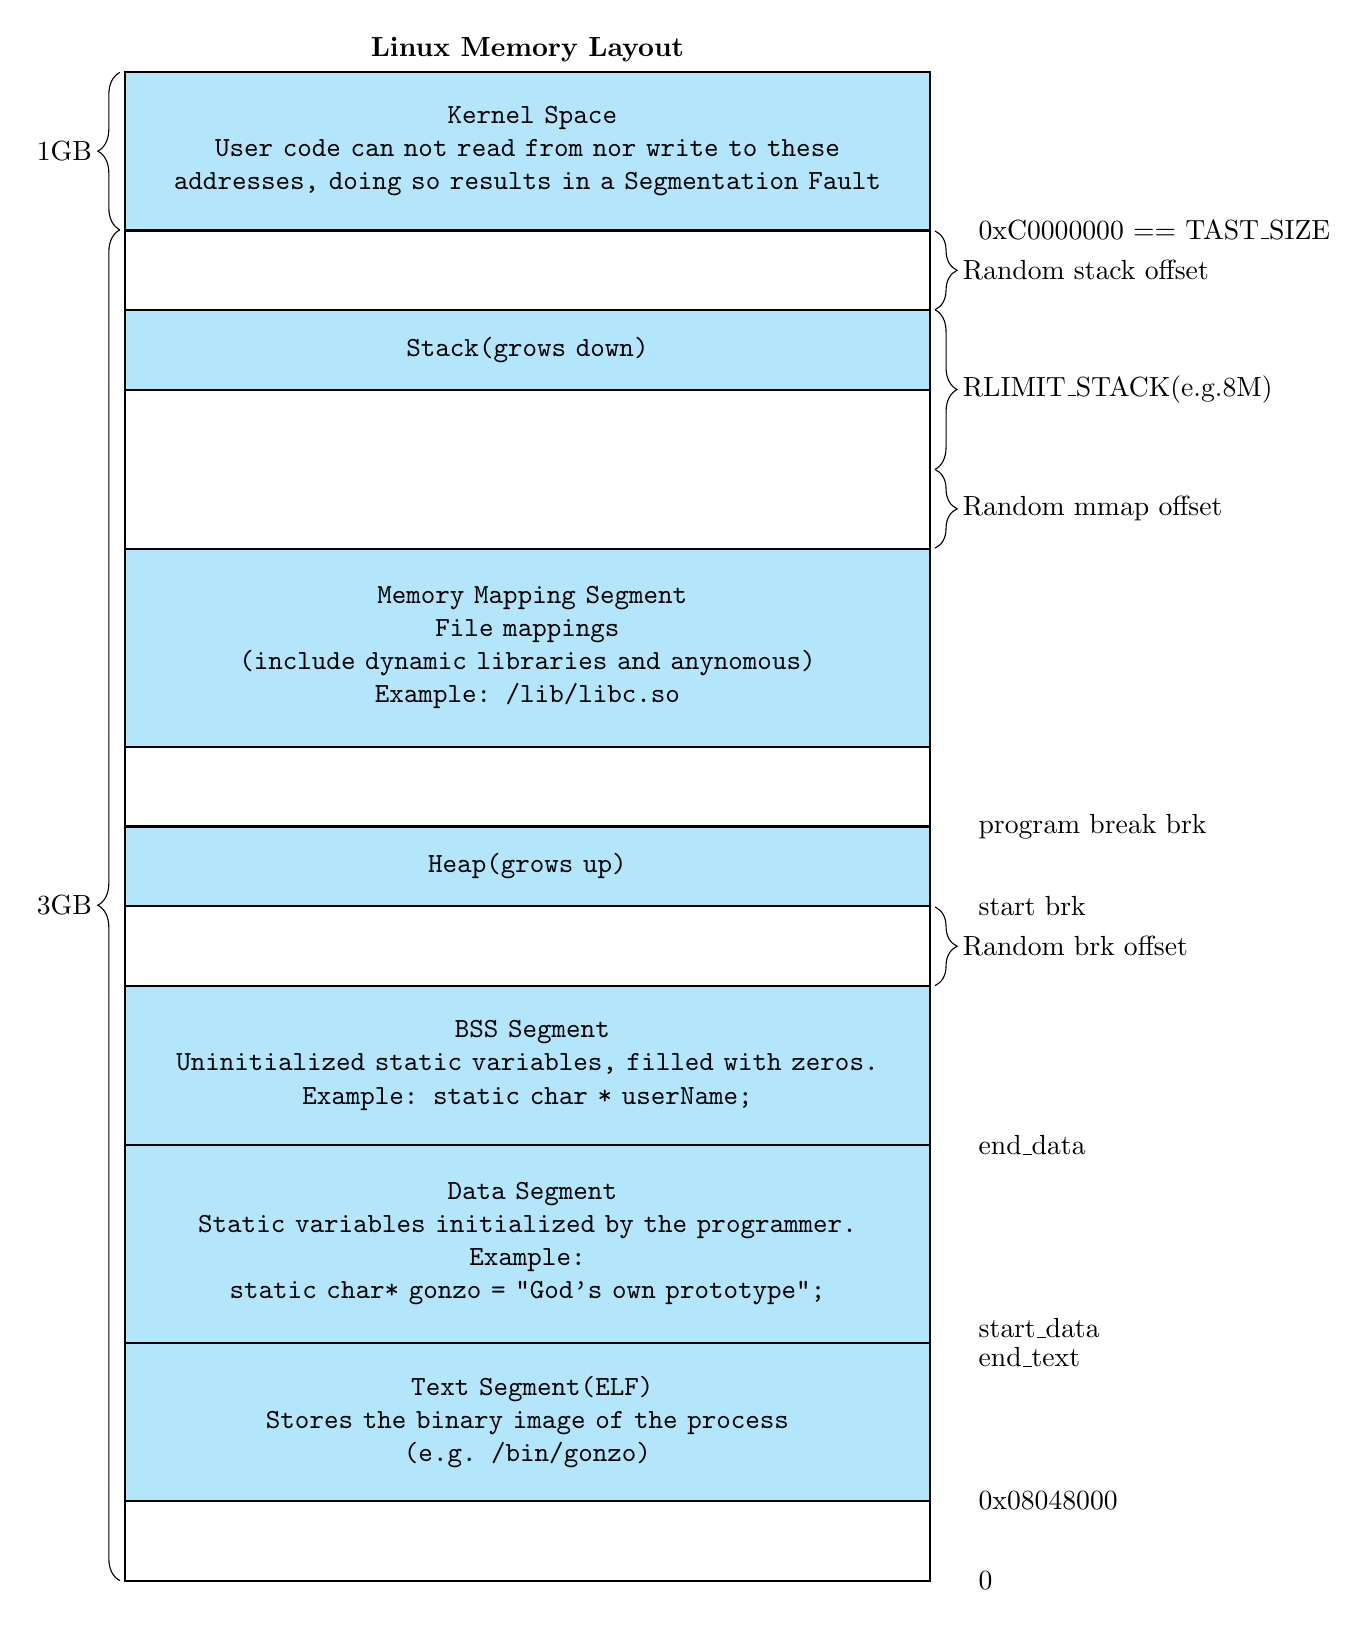
\begin{tikzpicture}

    \matrix (layout) [table={10cm}{Linux Memory Layout}] {
        |[non blank cell=2cm](kernel space)| {
            \textbf{Kernel Space}\\
            User code can not read from nor write to these\\
            addresses, doing so results in a Segmentation Fault}\\ % kernel space
        |[blank cell](stack offset)|{}\\ % random stack offset
        |[non blank cell=1cm]|{\textbf{Stack}(grows down)}\\ % stack
        |[blank cell,minimum height=2cm](mmap offset)|{}\\ % random mmap offset
        |[non blank cell=2.5cm]|{
            \textbf{Memory Mapping Segment}\\
            File mappings\\
            (include dynamic libraries and anynomous)\\
            Example: /lib/libc.so}\\ % memory mapping segment
        |[blank cell]|{}\\ %
        |[non blank cell=1cm](heap)|{\textbf{Heap}(grows up)}\\ % heap
        |[blank cell](brk offset)|{}\\ % random brk offset
        |[non blank cell=2cm](bss)|{
            \textbf{BSS Segment}\\
            Uninitialized static variables, filled with zeros.\\
            Example: static char * userName;}\\ % bss
        |[non blank cell=2.5cm](data)|{
            \textbf{Data Segment}\\
            Static variables initialized by the programmer.\\
            Example: \\
            static char* gonzo = "God's own prototype";}\\ % data segment
        |[non blank cell=2cm](text)|{
            \textbf{Text Segment}(ELF)\\
            Stores the binary image of the process\\
            (e.g. /bin/gonzo)}\\ % text segment
        |[blank cell](user space)|{}\\
    };
    % comments
    \draw [left brace] (kernel space.north west) -- node[left note]{1GB} (kernel space.south west);
    \draw [left brace] (kernel space.south west) -- node[left note]{3GB} (user space.south west);
    \draw [right brace] (stack offset.north east) -- node[right note]{Random stack offset} (stack offset.south east);
    \draw [right brace] (stack offset.south east) -- node[right note]{RLIMIT_STACK(e.g.8M)} (mmap offset.east);
    \draw [right brace] (mmap offset.east) -- node[right note]{Random mmap offset} (mmap offset.south east);
    \draw [right brace] (brk offset.north east) -- node[right note]{Random brk offset} (brk offset.south east);
    \node[right addr note] at (kernel space.south east) {0xC0000000 == TAST_SIZE};
    \node[right addr note] at (heap.north east) {program break brk};
    \node[right addr note] at (heap.south east) {start brk};
    \node[right addr note] at (data.north east) {end_data};
    \node[right addr note] at ([yshift=.5em]data.south east) {start_data};
    \node[right addr note] at ([yshift=-.5em]text.north east) {end_text};
    \node[right addr note] at (text.south east) {0x08048000};
    \node[right addr note] at (user space.south east) {0};
\end{tikzpicture}
\end{document}
